\documentclass[12 pt]{article}
\usepackage[table]{xcolor}
\usepackage{pgfgantt}
\usepackage{setspace}
\usepackage{tabularx}
\onehalfspace


\author{Vanessa Braglia \\ \\ \textit{Advisor}: Prof. Olaf Schenk \\ \textit{Assistant}: Fabio Verbosio}
\title{\textbf{Project Proposal} \\ The Swiss Scientific Social Network}



\begin{document}
\maketitle 

\section*{Project Description}
\subsection*{Introduction}
A social network consists of a set of objects connected to each other by social relations. The best way to model social networks is using graphs (we can see an example in Figure 1): the objects (entities) are represented as nodes and the connections as edges between two different nodes. \\
\begin{figure} [h!]
\centering 
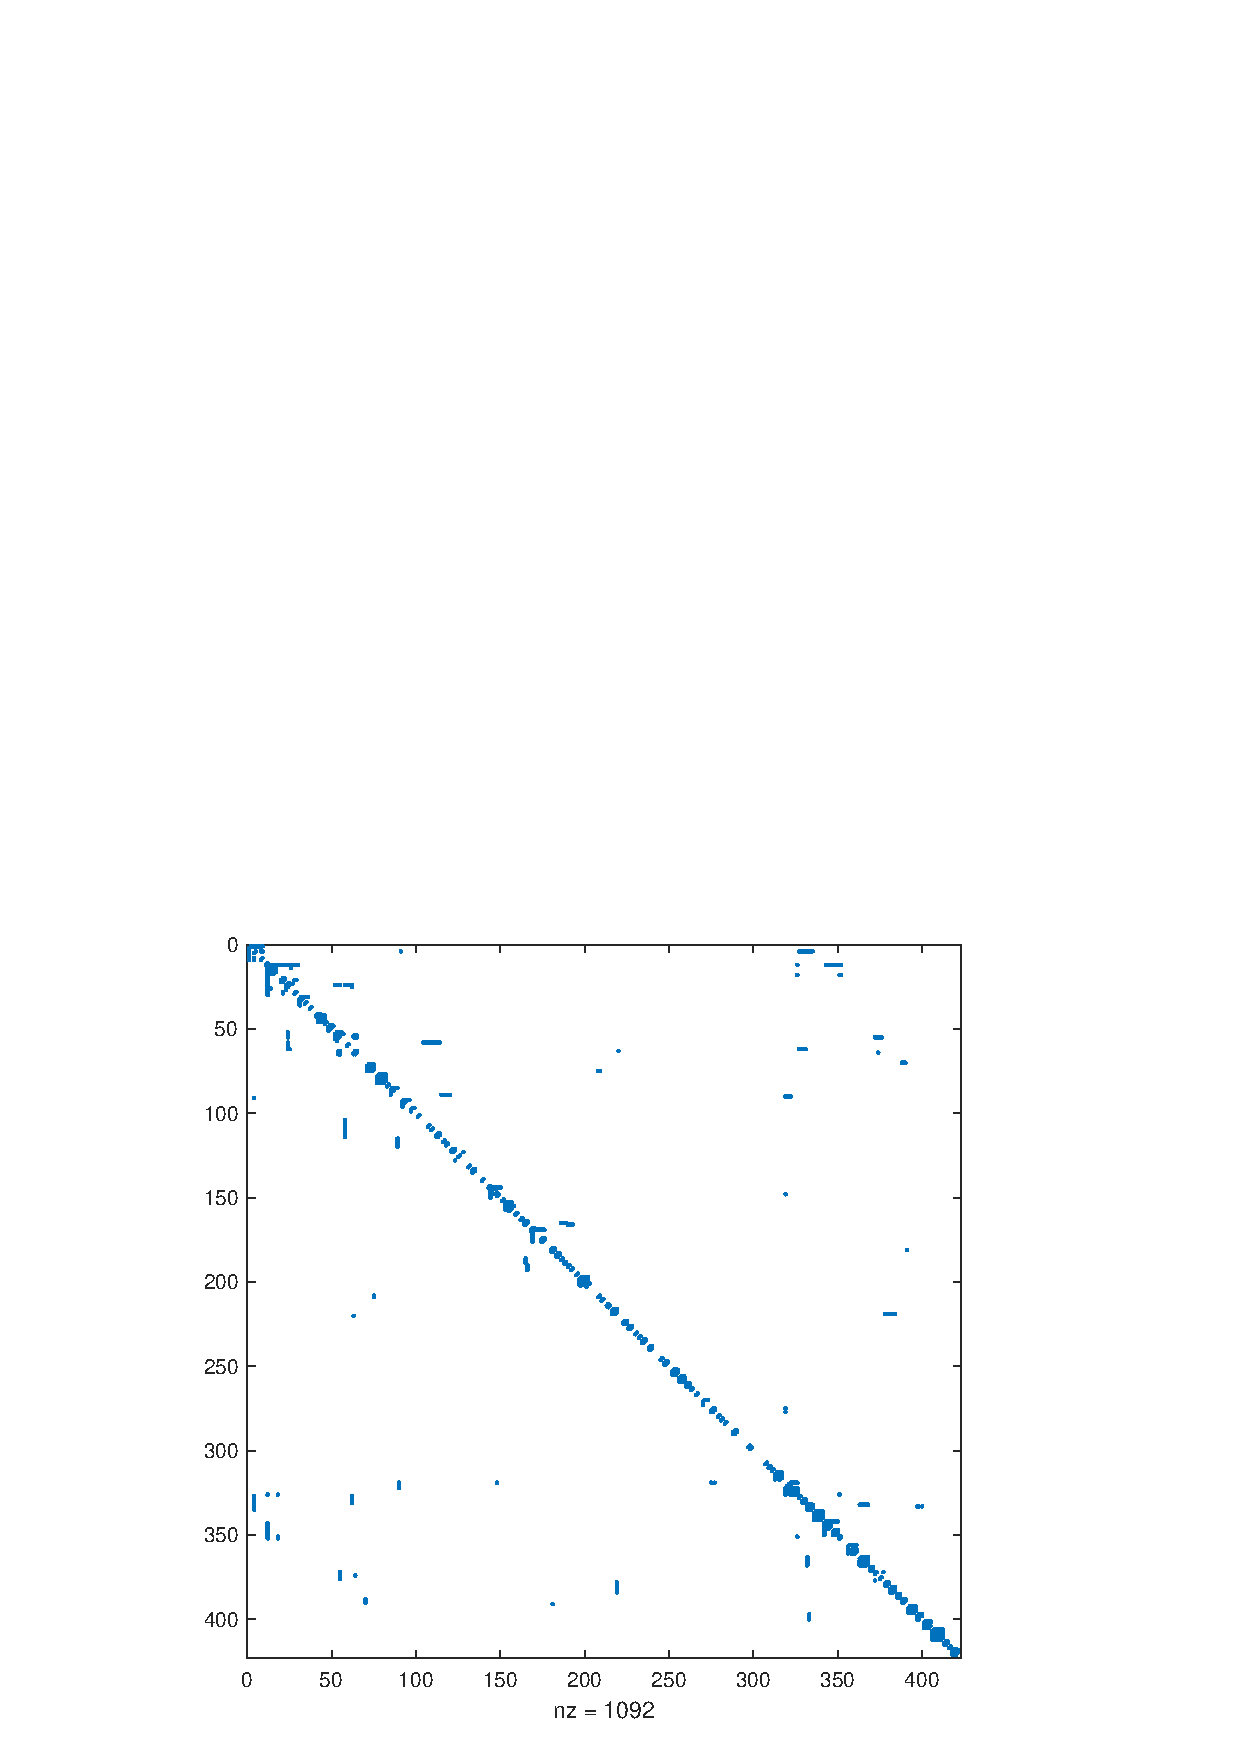
\includegraphics[scale=0.5]{graph.png}
\caption{Example of social network graph}
\end{figure}
The most common example we can take is the World Wide Web (WWW) where we have web pages as nodes connected by hyperlinks, the edges. In order to rank the huge amount of web pages and optimize the search for a particular page, more then twenty years ago was developed the PageRank (PR) algorithm. PageRank works on the graph representing the WWW, so it is applicable to all graphs representing social network.

\subsection*{Goal of the project}
The goal of this project is to create a social network of the scientific authors belonging to Swiss institutions, then analyze the relative graph and apply the PR algorithm.\\
The first step will be retrieving the information necessary for the construction of the social network based on coauthorship relations. Then there will be the implementation and application of the PageRank algorithm and the analysis of the graph.\\
The results will provide an interesting picture of the different research scenarios in Switzerland and how they interact with each other.

\subsection*{Implementation}
The first part of information retrieval will be done making requests to Mendeley API; the data obtained from this process will be filtered, to extract the information we need, and will be organized, to access easily to them.\\
The second part consists in analyzing all the information obtained: the PageRank algorithm will be implemented but we will use also other methods.\\
Graph Partitioning (we can see an example in Figure 2) will be useful to re-obtain the Swiss institutions based on the fact that members of the same institution will have more co-authorship relations with each other. \\
We will also visualize the connectivity matrices of the institutions and study their structures; looking at the cliques present in the matrices  we can for example detect the different research areas of the institutions and the connection between them.

\begin{figure} [h!]
\centering 
\includegraphics[scale=0.2]{graphPartitioning.png}
\caption{Example of graph partitioning}
\end{figure}

\section*{Milestones}
\begin{itemize}
\item[1.] Information retrieval
\item[2.] Data filtering
\item[3.]Data organization
\item[4.] Implementation of PR algorithm
\item[5.] Analysis of the information
\end{itemize}
\newpage
\section*{Time Table}
\begin{table}[ht]
\centering
\resizebox{\columnwidth}{!}{
\begin{tabular}{|l|c|c|c|c|c|c|c|c|c|c|c|c|c|c|}
\hline
\textit{Milestones} & 1 & 2 & 3 & 4 & 5 & 6& 7& 8& 9& 10& 11& 12& 13& 14\\
\hline
\hline
Information retrieval &\cellcolor{orange} &\cellcolor{orange}&\cellcolor{orange}&\cellcolor{orange}&\cellcolor{orange}&&&&&&&&&\\
\hline
Data filtering &&&&&&\cellcolor{orange}&\cellcolor{orange}&&&&&&&\\
\hline
Data organization &&&&&&&\cellcolor{orange}&\cellcolor{orange}&&&&&&\\
\hline
Implementation of PR algorithm &&&&&&&&& \cellcolor{orange} & \cellcolor{orange} &&&&\\
\hline
 Analysis of the information& &&&&&&&&&&\cellcolor{orange}&\cellcolor{orange}&\cellcolor{orange}&\\
 \hline
Project thesis& &&&&&&&&\cellcolor{orange}&\cellcolor{orange}&\cellcolor{orange}&\cellcolor{orange}&\cellcolor{orange}&\cellcolor{orange}\\
 \hline
Project poster& &&&&&&&&&&&&\cellcolor{orange}&\cellcolor{orange}\\
\hline
\end{tabular}
}
\end{table}
\end{document}
